\section{ANALYSIS AND RESULTS}

To study the socio-technical congruence of Cargo, I started analysing its package dependency network and the associated technical and social (commenting) activities of its GitHub contributors.
%For this purpose I used Python notebooks and relied on existing data analytics and statistical libraries.
Focusing on the research questions of Section~\ref{sec:intro}, I report some very preliminary analysis below.
For now, the presented results are anecdotal and need to be complemented with proper statistical hypothesis testing, survival analysis and prediction modeling.

I started to investigate how the commenting activity of contributors to a package relates to the introduction of a package dependency.
To do so, I considered all packages for which a new dependency was added at some point in time, and analysed whether commenting activity could be observed \emph{before} or \emph{after} depending on those packages.
Figure~\ref{fig:fig1} summarises the results. One can observe that more commenting activity happens on package repositories after the creation of dependencies to those packages than before adding such dependencies. 
An important shift in behaviour can be observed around September 2017, where the commenting activity before starting to depend on packages is increasing and an inverse trend shift is observed for the commenting activity after starting to depend on packages. Why this trend shift occurs remains an open question for now.

\begin{figure}[thb]
\vspace{-0.3cm}
    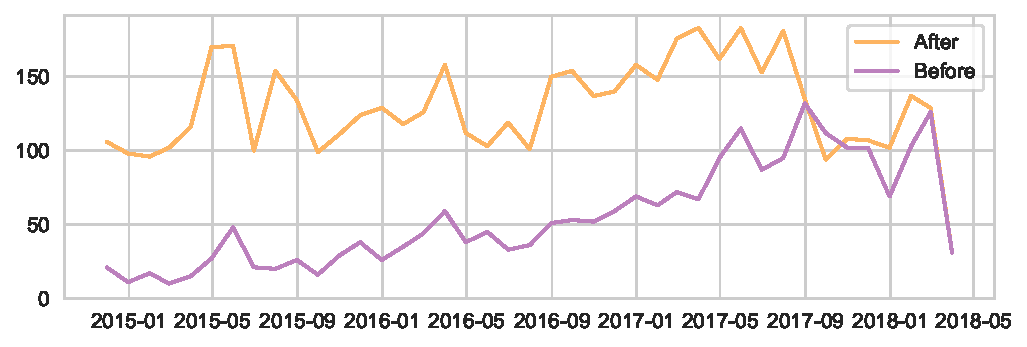
\includegraphics[width=0.9\columnwidth]{Photos/RQ21.pdf} 
    \caption{Commenting activity (number of comments) to package repositories before and after starting to depend on a package.}
    \label{fig:fig1}
\end{figure}

In order to assess which types of comments are more likely to lead to the introduction of new package dependencies, I analysed the proportion of comment types for all comments made in repositories of packages prior to the addition of a dependency to those packages. Figure~\ref{fig:fig2} presents these results. 
One can observe that, among the four types of comments considered (i.e., commit comments, issue comments, pull request comments and pull request review comments), the proportion of comments on pull requests and issue requests is considerably higher than for commit comments and review comments. I hypothesise that commenting on pull requests and issue requests for a package could serve as a good predictor for adding new dependencies to that package.

\begin{figure}[htb]
    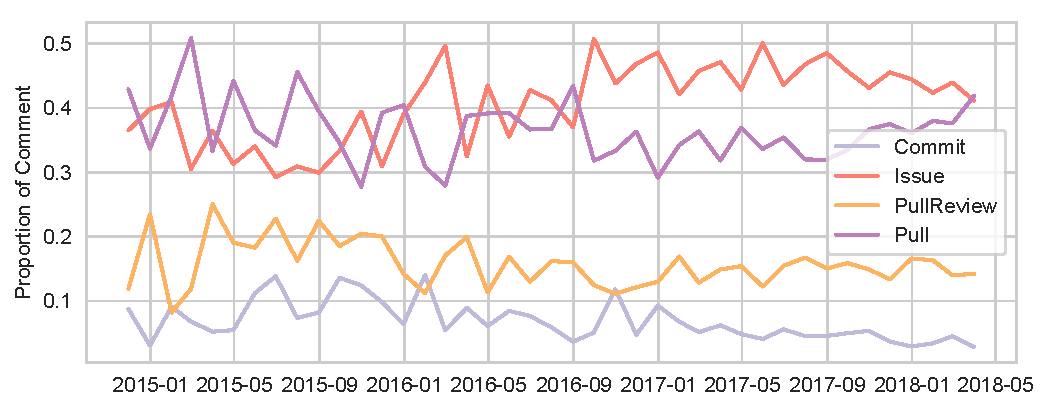
\includegraphics[width=0.9\columnwidth]{Photos/RQ22.pdf} 
    \caption{Proportion of comment types made in the repositories of packages before starting to depend on that package.}
    \label{fig:fig2}
\end{figure}

I also started to investigate whether social (i.e., commenting) activity on a package repository increases the likelihood to become technically active on that repository (i.e., submitting commits or pull requests). 
Figure~\ref{fig:fig3} presents some preliminary results. Considering the four different types of commenting activity, one can observe that issue comments are more likely to result in becoming technically active on a package repository.

\begin{figure}[thb]
    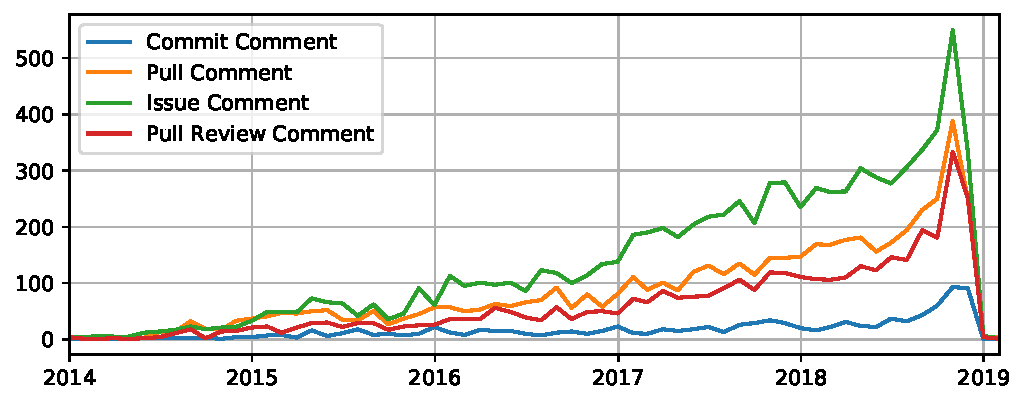
\includegraphics[width=0.9\columnwidth]{Photos/RQ3.pdf} 
    \caption{Number of comments (broken down by comment type) before starting  to technically contribute to a package.}
    \label{fig:fig3}
\end{figure}


